%%%%%%%% ICML 2026 EXAMPLE LATEX SUBMISSION FILE %%%%%%%%%%%%%%%%%

\documentclass{article}

% Recommended, but optional, packages for figures and better typesetting:
\usepackage{microtype}
\usepackage{graphicx}
\usepackage{subcaption}
\usepackage{array}
\usepackage{booktabs} % for professional tables
\usepackage{cuted}
\usepackage{tabularx}
\usepackage[section]{placeins}

% hyperref makes hyperlinks in the resulting PDF.
% If your build breaks (sometimes temporarily if a hyperlink spans a page)
% please comment out the following usepackage line and replace
% \usepackage{icml2026} with \usepackage[nohyperref]{icml2026} above.
\usepackage{hyperref}


% Attempt to make hyperref and algorithmic work together better:
\newcommand{\theHalgorithm}{\arabic{algorithm}}
\newcolumntype{Y}{>{\raggedright\arraybackslash}X}
\newcommand{\promptblock}[3]{%
  \subsection*{\texttt{#1}}
  \begingroup
  \small
  \setlength{\tabcolsep}{6pt}
  \renewcommand{\arraystretch}{1.15}
  \noindent\begin{tabularx}{\linewidth}{@{}>{\bfseries}p{0.17\linewidth}Y@{}}
  System & #2 \\
  User & #3 \\
  \end{tabularx}
  \par\endgroup\medskip
}
\setlength{\stripsep}{10pt plus 2pt minus 2pt}

% Use the following line for the initial blind version submitted for review:
% \usepackage{icml2026}

% For preprint, use
% \usepackage[preprint]{icml2026}

% If accepted, instead use the following line for the camera-ready submission:
\usepackage[accepted]{icml2026}

\usepackage{amsmath}
\usepackage{amssymb}
\usepackage{mathtools}
\usepackage{amsthm}


% if you use cleveref..
\usepackage[capitalize,noabbrev]{cleveref}

%%%%%%%%%%%%%%%%%%%%%%%%%%%%%%%%
% THEOREMS
%%%%%%%%%%%%%%%%%%%%%%%%%%%%%%%%
\theoremstyle{plain}
\newtheorem{theorem}{Theorem}[section]
\newtheorem{proposition}[theorem]{Proposition}
\newtheorem{lemma}[theorem]{Lemma}
\newtheorem{corollary}[theorem]{Corollary}
\theoremstyle{definition}
\newtheorem{definition}[theorem]{Definition}
\newtheorem{assumption}[theorem]{Assumption}
\theoremstyle{remark}
\newtheorem{remark}[theorem]{Remark}

% Todonotes is useful during development; simply uncomment the next line
%    and comment out the line below the next line to turn off comments
\usepackage[disable,textsize=tiny]{todonotes}

% The \icmltitle you define below is probably too long as a header.
% Therefore, a short form for the running title is supplied here:
\icmltitlerunning{Detecting hidden chain-of-thought in LLMs}

\begin{document}

\twocolumn[
  \icmltitle{Detecting hidden chain-of-thought in large language models with linguistic, behavioral, and mechanistic indicators}

  % It is OKAY to include author information, even for blind submissions: the
  % style file will automatically remove it for you unless you've provided
  % the [accepted] option to the icml2026 package.

  % List of affiliations: The first argument should be a (short) identifier you
  % will use later to specify author affiliations Academic affiliations
  % should list Department, University, City, Region, Country Industry
  % affiliations should list Company, City, Region, Country

  % You can specify symbols, otherwise they are numbered in order. Ideally, you
  % should not use this facility. Affiliations will be numbered in order of
  % appearance and this is the preferred way.
\icmlsetsymbol{equal}{*}

\begin{icmlauthorlist}
    \icmlauthor{Armaan Singh}{yyy}
    \icmlauthor{Ryan Trinh Le}{yyy}
    \icmlauthor{Jasmine Kaur}{yyy}
    \icmlauthor{Edward Lue Chee Lip}{}
    \icmlauthor{Kiran Nijjer}{yyy}
    \icmlauthor{Adnan Ahmed}{sch}
    \icmlauthor{Vasu Sharma}{fb}
\end{icmlauthorlist}

\icmlaffiliation{yyy}{Stanford University}
\icmlaffiliation{sch}{York University}
\icmlaffiliation{fb}{Facebook}

\icmlcorrespondingauthor{Armaan Singh}{armaan30312@gmail.com}

\icmlkeywords{Machine Learning, ICML}

  \vskip 0.3in
]

% this must go after the closing bracket ] following \twocolumn[ ...

% This command actually creates the footnote in the first column listing the
% affiliations and the copyright notice. The command takes one argument, which
% is text to display at the start of the footnote. The \icmlEqualContribution
% command is standard text for equal contribution. Remove it (just {}) if you
% do not need this facility.

% Use ONE of the following lines. DO NOT remove the command.
% If you have no special notice, KEEP empty braces:
\printAffiliationsAndNotice{~}
% Or, if applicable, use the standard equal contribution text:
% \printAffiliationsAndNotice{\icmlEqualContribution}

\begin{abstract}
Large language models often answer complex reasoning questions correctly without revealing intermediate steps, raising the question of whether they perform latent reasoning or pattern completion. Existing detection methods rely on surface-level linguistic cues that prior work has shown can be unfaithful. We propose the Hidden CoT Detection Score (HCDS), a comparative behavioral and mechanistic signal that quantifies whether a model's neutral-prompt behavior aligns more closely with its explicit-CoT or with its explicit no-CoT behavior. On Qwen3-4B Instruct, HCDS is robustly positive on both GSM8K and StrategyQA ($+1.87$ to $+2.38$, $p < 10^{-9}$) --- our cleanest hidden-CoT detection result. On Qwen3-4B Thinking, HCDS is also positive ($+0.33$ to $+0.60$, $p < 0.05$) but the result is better read as evidence of prompt-invariance of reasoning traces: under explicit no-CoT directives, Thinking emits a mean of ${\sim}575$ reasoning tokens vs Instruct's ${\sim}24$, so the no-CoT pole is not a clean answer-only baseline for that model. Anchor-suppression analysis further shows that the Thinking model distributes its causal load across many reasoning steps, suggesting that hidden chain-of-thought in reasoning-tuned models is more deeply integrated, more prompt-invariant, and more diffuse than in instruction-tuned ones.
\end{abstract}

\section{Introduction}

Explicit Chain of Thought (CoT) prompting improves LLM performance and exposes interpretable reasoning steps~\citep{wei_chain--thought_2023}, but it is unclear whether models engage in latent or implicit CoT reasoning when users do not request step-by-step output. Current methods identify implicit CoT only through surface-level cues and behavioral patterns. These cues are correlational, not causal. Misidentifying such patterns as reasoning weakens interpretability and erodes user trust.

Models can plausibly produce forms of reasoning text that do not contribute to the final output~\citep{turpin_language_2023}. Distinguishing the two necessitates understanding whether the visible steps causally created the answer or simply accompany it. Output-only analysis cannot achieve this, because genuine step-by-step reasoning and post-hoc rationalization of an already-determined answer can yield the same surface text; the evidence that would separate them lies in the internal computation, not the output.

We reframe latent reasoning detection from a correlational analysis of model outputs into a behavioral identification problem. We propose the Hidden CoT Detection Score (HCDS), which quantifies the extent to which a model's neutral-prompt behavior resembles its explicit reasoning patterns. HCDS is computed by systematically comparing model behavior across explicit CoT, explicit no-CoT, and neutral prompts along three feature families: linguistic signals comprising mean token entropy and entropy slope; behavioral signals comprising latency per output token, paraphrase consistency, and perturbation sensitivity; and a mechanistic signal measuring intervention sensitivity from internal activations and attention patterns in open-weight models. Output length is recorded only for diagnostic and length-matched analyses and is not included in the HCDS feature vector. The mechanistic signal additionally supports targeted interventions that selectively disrupt internal dependencies, allowing us to evaluate whether specific steps causally contribute to the model's output rather than merely accompany it.

We evaluate HCDS on Qwen3-4B (Instruct and Thinking variants) using GSM8K and StrategyQA, comparing each model's behavior across the three prompt conditions. HCDS is significantly positive for both models under neutral prompting on both datasets (GSM8K: +2.254 for Instruct, p = 2.21e-10; +0.479 for Thinking, p = 2.06e-02; StrategyQA: +1.871 for Instruct, p = 3.53e-12; +0.597 for Thinking, p = 2.15e-03), indicating that neutral behavior aligns more closely with explicit CoT than with explicit no-CoT. The Instruct effect is robust across feature-ablation variants and across short, medium, and long questions; the Thinking effect is smaller and length-sensitive, weakening on medium-length questions where reasoning traces approach the generation cap. Anchor-suppression interventions further reveal that the Thinking model's explicit reasoning chains distribute causal load across many steps rather than concentrating in a few, an unexpected mechanistic finding the rest of the paper develops.


\section{Related Work}

A first line of related work asks whether visible chain-of-thought explanations faithfully reflect the computation that produces a model's answer. \citet{turpin_language_2023} show that chain-of-thought explanations can be unfaithful, in the sense that models may produce plausible reasoning text that is not causally responsible for their final prediction. More recently, \citet{chen_reasoning_2025} test faithfulness through controlled prompt-hint interventions and show that reasoning traces do not always transparently reveal what the model used to reach its answer. These works motivate the central premise of our paper: output-only inspection is insufficient for determining whether reasoning is occurring internally. Our contribution differs in scope and objective. Rather than asking whether an explicit rationale is faithful, we ask whether latent reasoning is occurring at all under neutral prompting, and we address this question through a combination of behavioral and mechanistic signals rather than through rationale analysis alone.

A second line of work studies whether latent reasoning exists as a genuine internal phenomenon. \citet{lin_implicit_2025} argue that implicit reasoning in Transformers often emerges through shortcut learning and can fail to generalize when problem structure changes, suggesting that correct answers without explicit CoT need not imply robust reasoning. Concurrent work by \citet{he_reasoning_2026} provides mechanistic evidence that latent reasoning corresponds to steerable internal features, showing that reasoning behavior can be activated without explicit chain-of-thought prompting. These papers establish that latent reasoning is both real and difficult to interpret: it can exist as an internal computational mode, but may also be entangled with brittle heuristics. Our work differs by proposing a detection framework for identifying when such latent reasoning is being used at inference time, rather than studying how it emerges during training or how it can be induced through latent steering.

The work most closely related to our mechanistic component is \citet{bogdan_thought_2025}, who identify ``thought anchors'' --- reasoning steps within explicit CoT traces that have disproportionate influence on downstream generation. They propose black-box, attention-based, and causal attribution methods to determine which steps matter most within a visible reasoning chain. Our paper builds on this intervention logic but shifts the question from which explicit reasoning steps matter to whether reasoning is happening under neutral prompting at all. In our framework, anchor-based perturbation is not the end goal but one feature family within a broader hidden-CoT detection score. This difference is important: Bogdan et al. analyze the internal structure of explicit CoT, whereas we use related mechanistic tools to detect latent reasoning in the absence of explicit CoT.

\section{Background}

Our method builds on prior work in Transformer language models, chain-of-thought prompting, reasoning benchmarks, and causal interpretability. Because the goal of this paper is to detect hidden chain-of-thought reasoning rather than to elicit it directly, the relevant background is not only how reasoning prompts improve model performance, but also how internal computations in Transformer models can be analyzed through interventions.

Modern large language models are based on the Transformer architecture introduced by \citet{vaswani_attention_2023}. The Transformer replaces recurrence with stacked self-attention and feedforward layers, making token-level contextual interactions, residual-stream representations, and layerwise interventions central objects of analysis. These architectural components are directly relevant to our method because the mechanistic part of our framework studies internal activations and intervention effects within a Transformer model.

The prompting side of our framework is inherited from chain-of-thought prompting. \citet{wei_chain--thought_2023} showed that prompting a language model to produce intermediate reasoning steps can substantially improve performance on multi-step reasoning tasks. In our setting, explicit CoT prompting serves as one anchor condition, while explicit no-CoT prompting serves as a contrasting answer-only condition. Our objective is not to improve reasoning through prompting itself, but to use these prompt conditions as reference points for determining whether a model under a neutral prompt behaves more like an overt reasoner or more like a direct-answer generator.

Our experiments are grounded in two reasoning benchmarks. GSM8K, introduced by \citet{cobbe_training_2021}, is a benchmark of grade-school mathematical word problems designed to test multi-step arithmetic reasoning. StrategyQA, introduced by \citet{geva_did_2021}, is a benchmark of yes/no questions that require implicit multi-hop commonsense reasoning. Together, these datasets allow us to evaluate hidden-CoT detection across both quantitative and qualitative reasoning settings while keeping the tasks sufficiently structured for prompt-matched comparisons.

The mechanistic component of our framework draws on causal intervention methods in interpretability. \citet{meng_locating_2023} showed that targeted manipulation of internal activations can identify and alter computationally important representations in autoregressive Transformer language models. This intervention-based perspective provides the conceptual basis for our anchor-suppression analysis: if perturbing a candidate reasoning-relevant internal state changes the final answer more than a matched control intervention, then that state is likely to play a causal role in the model's solution process.

\subsection{Problem Setting}

We study hidden chain-of-thought as a comparative detection problem. For a fixed model and question, we observe behavior under three prompt conditions: explicit CoT, explicit no-CoT, and neutral. Let $f_{m,q,p}$ denote the feature vector for model $m$, question $q$, and prompt condition $p$. Our method asks whether the neutral feature vector is closer to the explicit-CoT feature vector or to the explicit-no-CoT feature vector. Positive alignment with explicit CoT is interpreted as evidence that the model relies on latent intermediate reasoning even when that reasoning is not explicitly shown.

\section{Method}

\begin{figure*}[!t]
  \centering
  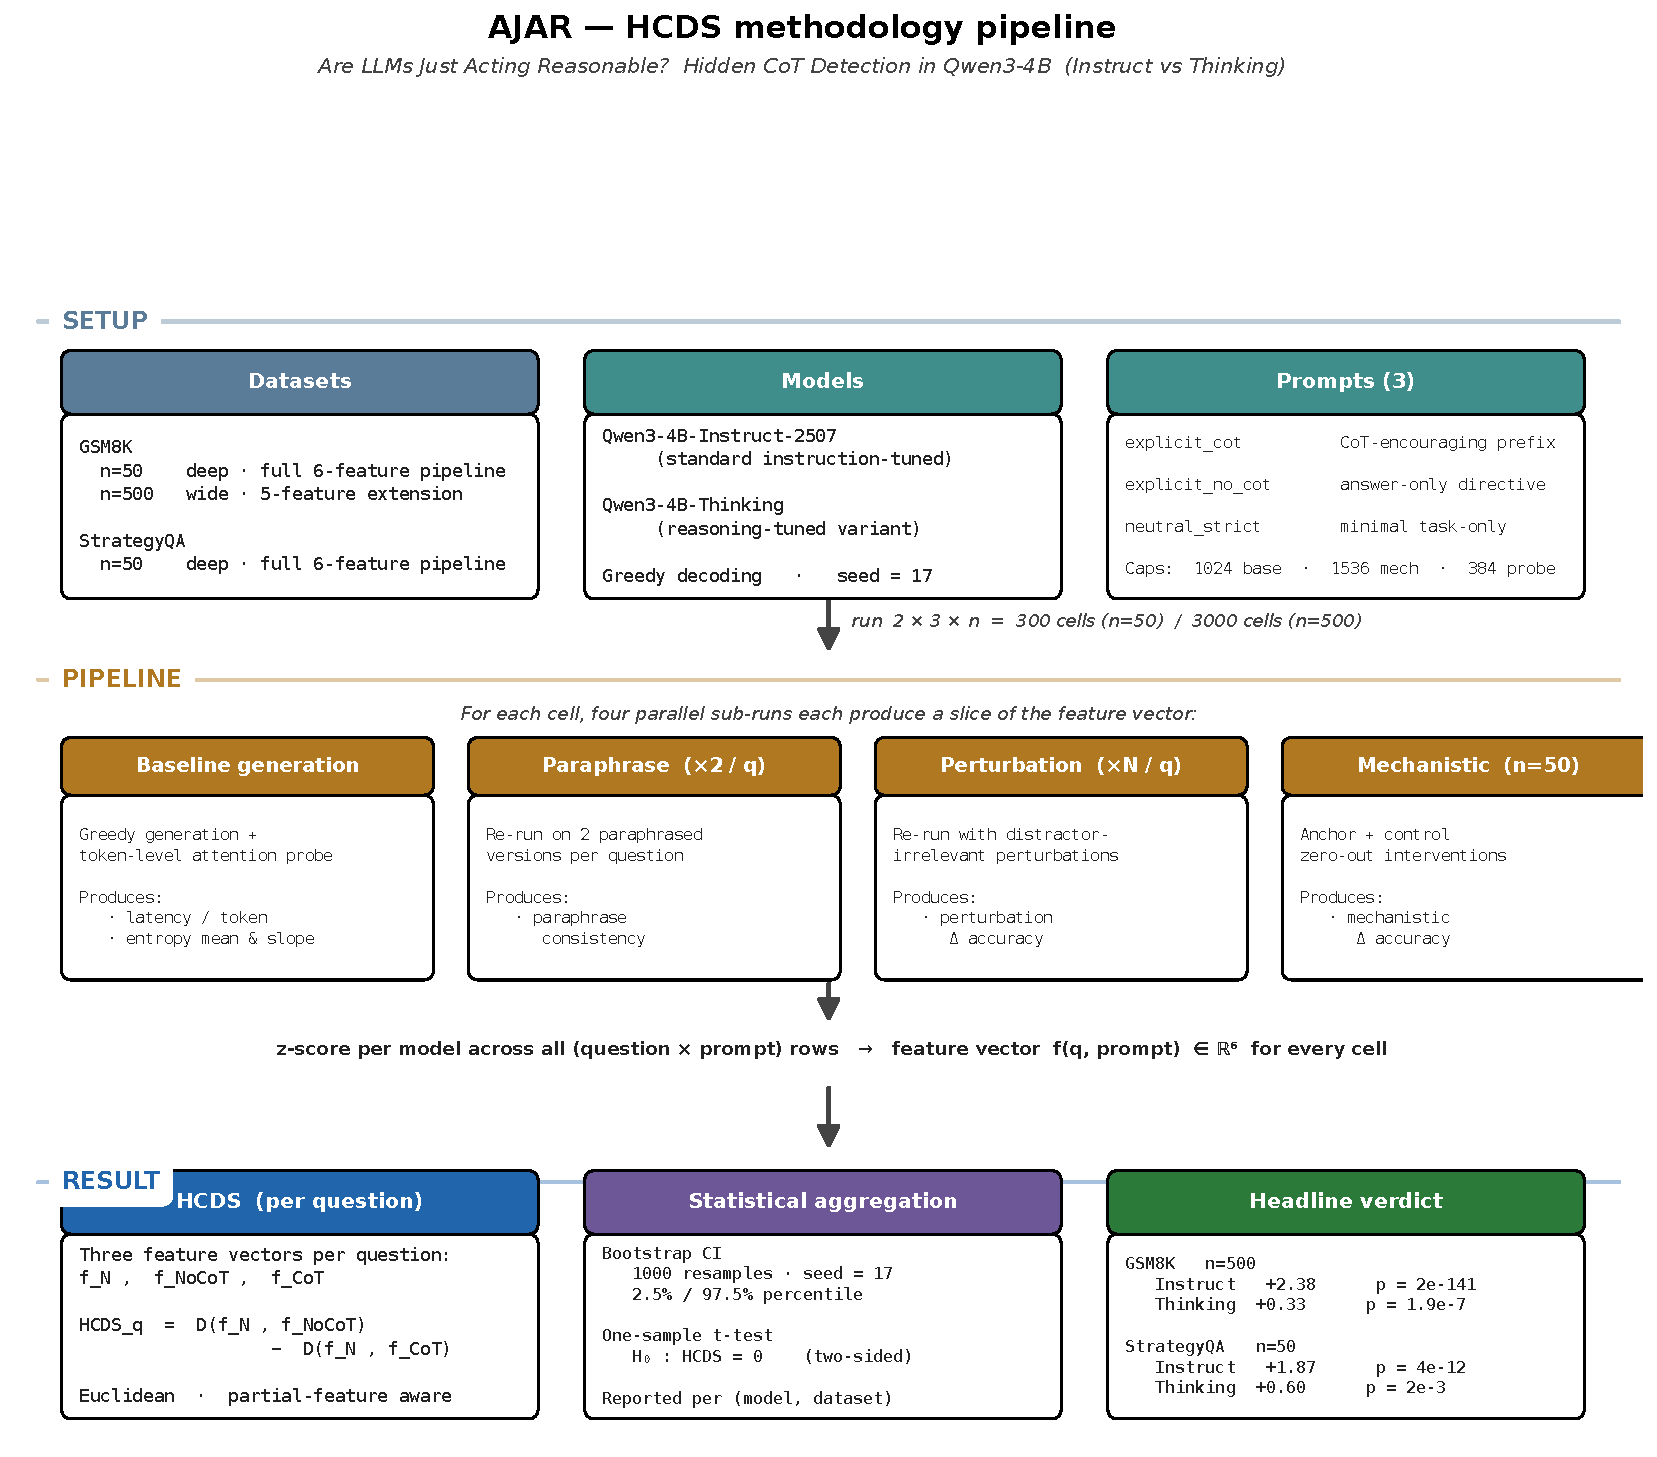
\includegraphics[width=\textwidth]{figures/fig0_methods_pipeline.pdf}
  \caption{\textbf{HCDS methodology pipeline.}
  \textit{Setup:} two datasets $\times$ two models $\times$ three
  prompts.
  \textit{Pipeline:} for each $(\mathrm{model}, \mathrm{prompt}, \mathrm{question})$
  cell, four parallel sub-pipelines (baseline + attention probe,
  paraphrase, perturbation, mechanistic) produce a six-dimensional
  feature vector that is z-scored per model.
  \textit{Result:} HCDS contrasts the neutral prompt's distance to
  the no-CoT pole vs the CoT pole, with bootstrap CIs and a
  one-sample two-sided t-test reported per $(\mathrm{model}, \mathrm{dataset})$.
  Sign of HCDS distinguishes hidden reasoning ($>0$), ambiguity
  ($\approx 0$), and no hidden reasoning ($<0$); observed values
  appear in Figure~\ref{fig:cross-dataset}.}
  \label{fig:methods}
\end{figure*}

We formulate hidden chain-of-thought (CoT) detection as a comparative inference problem. Figure~\ref{fig:methods} summarizes the full workflow. For each model $m$ and question $q$, we evaluate three prompt conditions: \textit{explicit\_cot}, which asks the model to reason step by step; \textit{explicit\_no\_cot}, which asks for a direct answer without reasoning; and \textit{neutral\_strict}, a minimal task-only prompt that gives no instruction about whether reasoning should be shown. Full prompt text is provided in Appendix~\ref{app:prompts}. Rather than attempting to recover an internal reasoning trace directly, we ask whether the model's behavior under the neutral prompt is closer to its behavior under explicit CoT or explicit no-CoT. For each $(m,q,p)$ tuple, we construct a feature vector
\[
\begin{aligned}
f_{m,q,p} = \bigl[&\ell_{m,q,p},\; \bar{H}_{m,q,p},\; s^{H}_{m,q,p},\; C^{\mathrm{para}}_{m,q,p},\\
&\Delta A^{\mathrm{pert}}_{m,q,p},\; \Delta A^{\mathrm{mech}}_{m,q,p}\bigr].
\end{aligned}
\]
where the components denote latency per output token, mean token entropy, entropy slope, paraphrase consistency, perturbation sensitivity, and mechanistic intervention sensitivity.

We compare prompt conditions by Euclidean distance in z-scored feature space. When some features are unavailable for a given question, we compute distances only over the shared observed dimensions $\mathcal{J}_q$:
\[
D(a,b) = \sqrt{\sum_{j \in \mathcal{J}_q} (a_j - b_j)^2}.
\]
We then define the per-question Hidden CoT Detection Score (HCDS). Intuitively, $\mathrm{HCDS}_q > 0$ means the model's neutral-prompt behavior on question $q$ looks more like its overt-CoT behavior than its overt no-CoT behavior --- i.e., the model is behaving as if it is reasoning under the hood. Formally:
\begin{equation}
\begin{aligned}
\mathrm{HCDS}_q ={}& D\!\left(f_{m,q,\mathrm{neutral}}, f_{m,q,\mathrm{no\text{-}cot}}\right) \\
&- D\!\left(f_{m,q,\mathrm{neutral}}, f_{m,q,\mathrm{cot}}\right).
\end{aligned}
\label{eq:hcds-q}
\end{equation}
A positive $\mathrm{HCDS}_q$ indicates that the model's neutral-prompt behavior is closer to explicit CoT than to explicit no-CoT for that question, which we interpret as evidence of hidden reasoning.

At the model--dataset level, we aggregate per-question scores as
\begin{equation}
\overline{\mathrm{HCDS}} = \frac{1}{N}\sum_{q=1}^{N} \mathrm{HCDS}_q.
\label{eq:hcds-mean}
\end{equation}
This framing treats hidden CoT as a functional dependency on intermediate computation rather than a visible linguistic artifact. The behavioral features capture whether neutral prompting exhibits the timing, uncertainty, and consistency profile expected of overt reasoning, while the mechanistic feature tests whether suppressing candidate reasoning \emph{anchors} (the reasoning steps our attention/activation proxies flag as most causally influential, defined operationally in Section~\ref{sec:results-mech}) harms performance more than matched control interventions. Together, these signals allow us to distinguish three regimes: neutral behavior that aligns with explicit CoT, neutral behavior that aligns with explicit no-CoT, and ambiguous cases where the evidence does not clearly support either interpretation.

\section{Experimental Setup}

We evaluate two open-weight models from the same family, Qwen3-4B-Instruct-2507 and Qwen3-4B-Thinking-2507, on GSM8K and StrategyQA. GSM8K tests multi-step arithmetic reasoning, while StrategyQA tests multi-hop commonsense reasoning with binary yes/no answers. We use the same three prompt conditions for both datasets: \textit{explicit\_cot}, \textit{explicit\_no\_cot}, and \textit{neutral\_strict} (the names used in our codebase and figures; for brevity we refer to them as explicit CoT, explicit no-CoT, and neutral throughout the prose). All main experiments use fixed decoding settings across conditions and deterministic decoding, so each question contributes one run per prompt condition and the question is the primary statistical unit. Because decoding is deterministic with one run per question, all reported confidence intervals and p-values quantify variation across questions, not sampling variability over stochastic model generations.


For each $(m,q,p)$ tuple, we record answer accuracy, generation time, output length, latency per output token, token-level entropy summaries, paraphrase consistency, perturbation delta accuracy, and mechanistic intervention delta accuracy when available. Answer accuracy and output length are auxiliary diagnostics; they do not enter the HCDS feature vector. The remaining measurements feed the comparative pipeline in Figure~\ref{fig:methods}. Latency per output token is defined as
\[
\ell_{m,q,p} = \frac{t^{\mathrm{gen}}_{m,q,p}}{T^{\mathrm{out}}_{m,q,p}},
\]
and token entropy is summarized by its mean and slope over the generated continuation:
\[
\begin{aligned}
\bar{H}_{m,q,p}
&=
\frac{1}{T^{\mathrm{out}}_{m,q,p}}
\sum_{t=1}^{T^{\mathrm{out}}_{m,q,p}}
H_t,
\\
H_t
&= -\sum_{v} p_t(v)\log p_t(v).
\end{aligned}
\]
We define the three content-level features concretely as follows. \emph{Paraphrase consistency} $C^{\mathrm{para}}$ is the fraction of $K$ meaning-preserving rewordings of the question on which the model returns the same answer it gave on the original; the rewordings are generated by a deterministic Qwen3-4B-Instruct paraphraser constrained to preserve every numeric value, the arithmetic structure, the named entities, and the gold answer. \emph{Perturbation sensitivity} $\Delta A^{\mathrm{pert}} = A_{\mathrm{orig}} - A_{\mathrm{pert}}$ is the accuracy drop under a \emph{distractor-irrelevant} perturbation: we insert a single irrelevant clause (e.g., ``The neighbor's dog barked seven times that afternoon.'') immediately before the final question sentence, leaving every quantity used in the gold reasoning chain untouched, so the correct answer is unchanged and any drop reflects fragility to surface distractors rather than a genuinely harder problem. \emph{Mechanistic sensitivity} $\Delta A^{\mathrm{mech}} = (A_{\mathrm{base}} - A_{\mathrm{anchor}}) - (A_{\mathrm{base}} - A_{\mathrm{control}})$ is the anchor-suppression contrast, i.e.\ the extra accuracy lost by zeroing out a trace's anchor steps beyond what is lost by zeroing out matched control steps; the anchor, control, and suppression procedures are defined operationally in Section~\ref{sec:results-mech} and specified in full in Appendix~\ref{app:mech-details}.

We report HCDS separately for each model and dataset, together with robustness analyses. We interpret HCDS primarily by its sign and statistical support: positive values indicate that neutral behavior is closer to explicit CoT than to explicit no-CoT, while values near zero indicate ambiguity. We do not assign a universal semantic meaning to raw HCDS magnitude, since it depends on the chosen z-scored feature space and feature coverage. Statistical evaluation tests
\[
H_0:\; \mathbb{E}[\mathrm{HCDS}_q] = 0
\qquad \text{vs.} \qquad
H_1:\; \mathbb{E}[\mathrm{HCDS}_q] \neq 0,
\]
using per-question scores, bootstrap confidence intervals, and question-level significance tests. To assess whether the signal is driven by a single feature or by output length alone, we additionally report leave-one-feature-out variants, single-feature variants such as entropy-only and latency-only HCDS, and length-matched analyses. For the open-weight models, we also summarize anchor-versus-control intervention results as mechanistic validation of the hidden-CoT signal.

\section{Results}

\begin{figure}[!htbp]
  \centering
  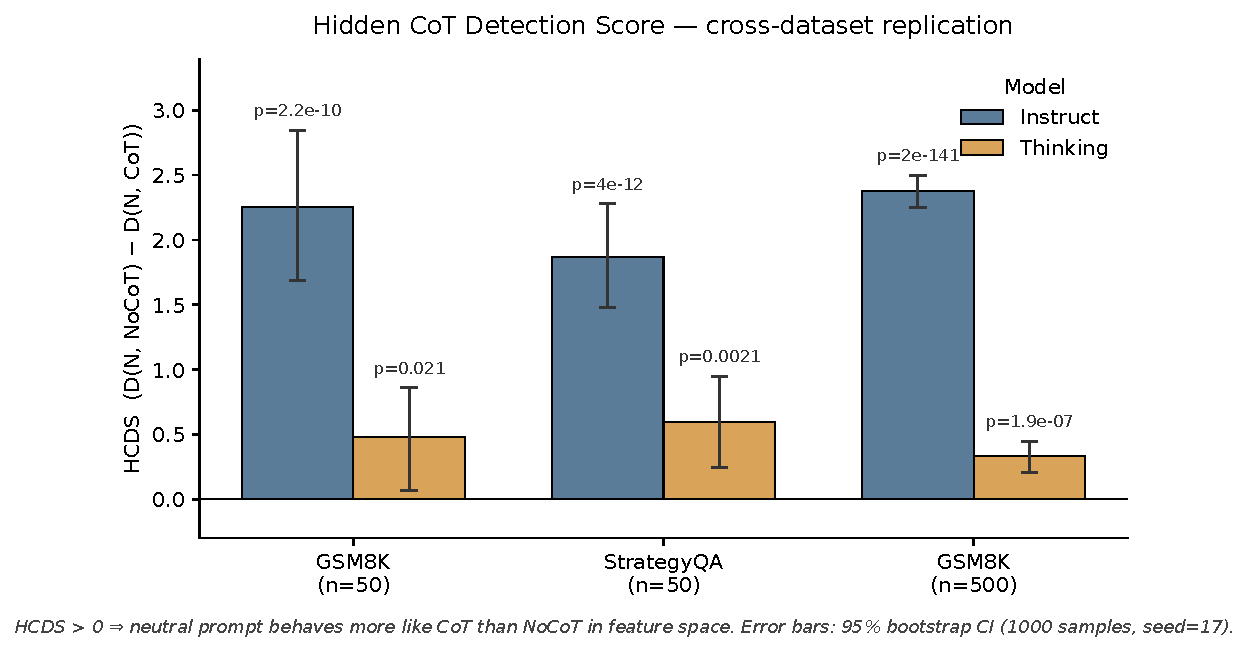
\includegraphics[width=\columnwidth]{figures/fig1_cross_dataset_hcds.pdf}
  \caption{\textbf{Cross-dataset HCDS replication.} HCDS is positive
  with $p < 0.05$ for both Qwen3-4B variants on both datasets and
  at both scales. Strongest question-level evidence: GSM8K $n{=}500$ Instruct
  ($p = 1.98\mathrm{e}{-141}$). Error bars: 95\% bootstrap CI
  (1000 samples, seed=17). Two-sided t-test p-values labeled
  above each bar.}
  \label{fig:cross-dataset}
\end{figure}

\subsection{Cross-Dataset Replication}

Figure~\ref{fig:cross-dataset} shows that the central HCDS result replicates across GSM8K and StrategyQA and strengthens further when GSM8K is scaled from $n=50$ to $n=500$. HCDS is significantly positive ($p < 0.05$) for both Qwen3-4B variants on both datasets and at both scales; the strongest question-level evidence is the GSM8K $n=500$ extension, where the Instruct model reaches $\overline{\mathrm{HCDS}} = +2.375$ with $p \approx 2 \times 10^{-141}$ (Eq.~\ref{eq:hcds-mean}). The Thinking signal is smaller in magnitude but consistently positive across all four (model, dataset) combinations. The consistent positive sign indicates that hidden-CoT detection is not captured by answer accuracy alone, but by the joint behavioral and mechanistic profile induced by the three prompt conditions.

\FloatBarrier
\subsection{Mechanistic Anchor Analysis}
\label{sec:results-mech}

\begin{figure*}[!t]
  \centering
  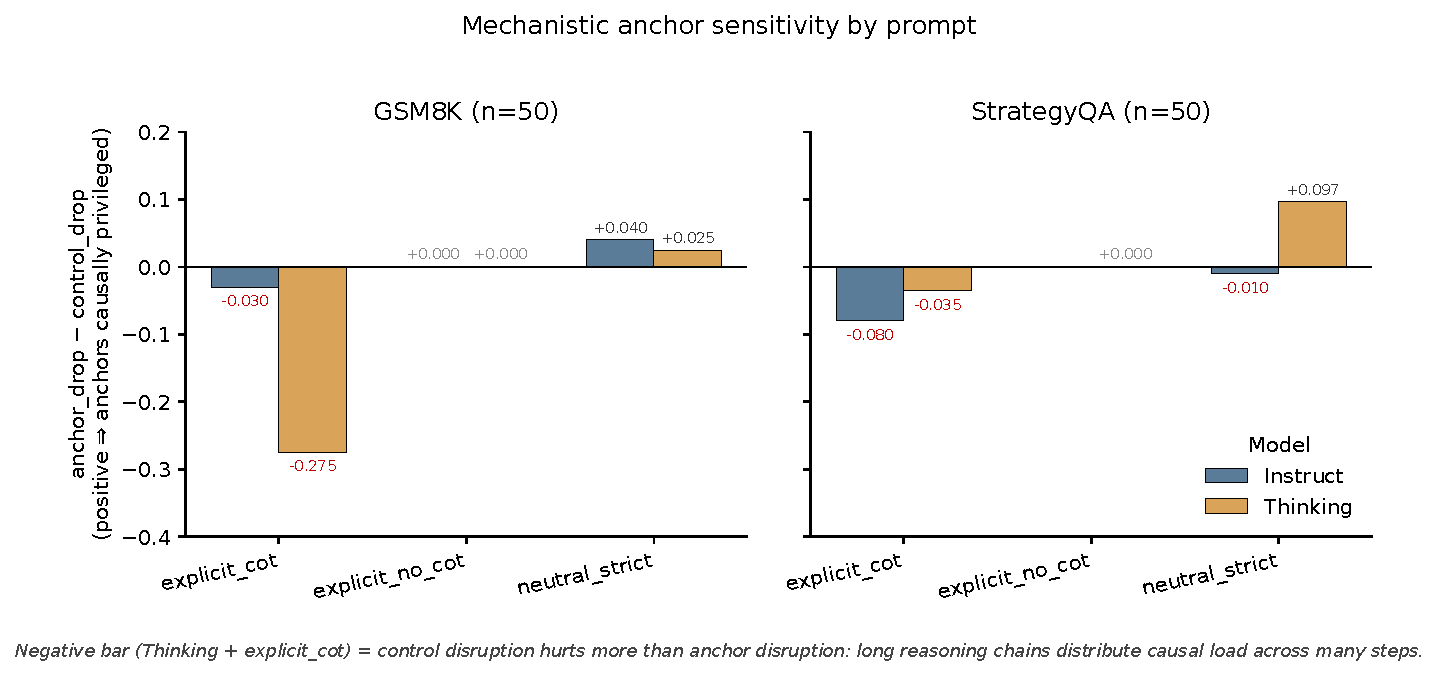
\includegraphics[width=\textwidth]{figures/fig4_anchor_control.pdf}
  \caption{\textbf{Anchor sensitivity.}
  $\mathrm{anchor\_drop} - \mathrm{control\_drop}$ across three
  prompt conditions on GSM8K and StrategyQA ($n{=}50$ each).
  Positive bars indicate anchors carry a privileged causal load;
  the negative Thinking + \texttt{explicit\_cot} bar on GSM8K
  ($-0.275$) is reported transparently --- long reasoning chains
  distribute causal load across many steps rather than
  concentrating it in a few attention anchors.}
  \label{fig:anchor}
\end{figure*}

Anchor interventions provide a mechanistic check on the behavioral score. We adopt the \emph{thought-anchor} notion of \citet{bogdan_thought_2025} --- a reasoning step that exerts disproportionate causal influence on the rest of the generation --- and operationalize it as follows. We segment each trace into reasoning steps and score every step on three attention-/activation-based proxies, all measured over the step's own generated tokens: \emph{forward-attention} (how much later reasoning steps attend back to it), \emph{answer-attention} (how much the final-answer span attends to it), and \emph{activation-delta} (the magnitude of the residual-stream change it induces). The top 2 steps by combined score are the \emph{anchors}; 1 random non-anchor step is the \emph{control}. We then \emph{suppress} a step by overwriting its contribution with zero during a re-decode: at the 4 step-specific layers that attend to it most, we multiply either the layer's residual-stream output (\texttt{residual\_zero}) or its attention-block output (\texttt{attention\_zero}) by zero at exactly that step's token positions --- and only those positions --- then resume greedy decoding from the prefix up to and including the suppressed step and re-parse the final answer ($2$ modes $\times$ ($2$ anchors $+$ $1$ control) $=$ 6 interventions per cell). If a step is causally load-bearing, zeroing it should reduce answer accuracy; \emph{anchor suppression} is this operation applied to the anchor steps, and $\Delta A^{\mathrm{mech}}$ (the anchor-minus-control accuracy drop) isolates the causal premium of anchors over arbitrary steps. Full per-cell counts and methodology details are in Appendix~\ref{app:mech-details}. Figure~\ref{fig:anchor} plots anchor-minus-control drops across prompt conditions on both datasets. Positive anchor-control contrasts indicate that identified anchors carry privileged causal load relative to the random-control baseline, which is the dominant pattern for Instruct. The notable exception is the Thinking model under \texttt{explicit\_cot} on GSM8K, where the anchor-control contrast is $-0.275$. We see two non-mutually-exclusive interpretations of this negative bar. First, long reasoning chains in the Thinking model may distribute causal dependence across many steps instead of concentrating it in a few dominant anchors --- consistent with the Thinking model's larger no-CoT output footprint discussed in Section~\ref{sec:discussion}. Second, our anchor-scoring formula combines forward-attention, answer-attention, and activation-delta proxies, all of which trend toward late-trace ``summary'' or ``answer-formulation'' steps in long traces; suppressing these post-hoc summary steps is less damaging than suppressing earlier mid-reasoning computation that downstream tokens have not yet copied. To partially disambiguate these interpretations, we ran a joint-suppression experiment that intervenes at \emph{both} top-2 anchor steps simultaneously and at a matched joint control of 2 random non-anchor steps (Appendix~\ref{app:joint-anchor}); the joint anchor-control contrast on Thinking + explicit\_cot moves from $-0.275$ (single) to $-0.120$ (joint), a 56\% narrowing of the negative gap. This partially supports the distributed-causal-load reading but also reveals that single random-control selection had inflated the original negative bar. We treat the development of position-matched controls and an anchor-scoring rule that is robust to long-trace summary bias as future work.

\FloatBarrier
\subsection{Robustness to Feature Choice}
\label{sec:robustness}

\begin{figure}[!htbp]
  \centering
  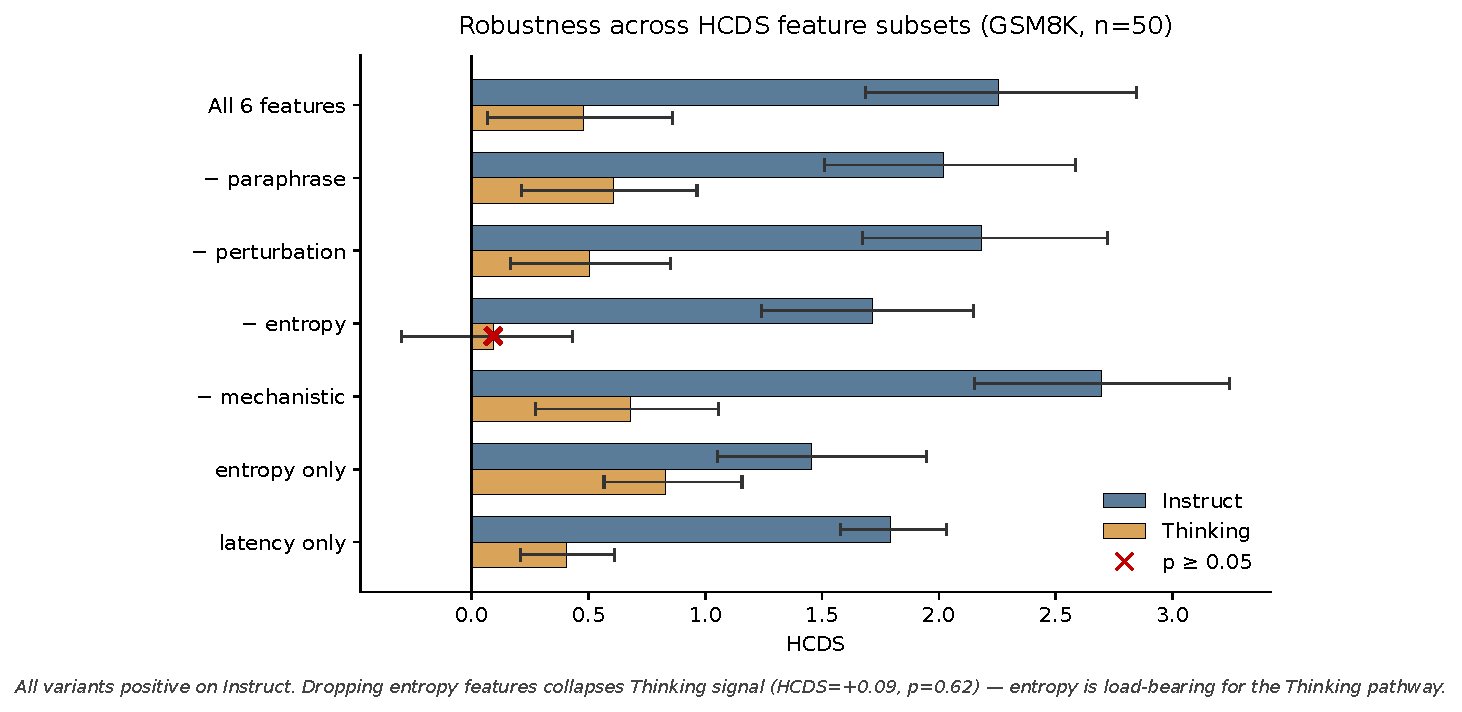
\includegraphics[width=\columnwidth]{figures/fig2_robustness_ablation.pdf}
  \caption{\textbf{Feature-ablation robustness.} HCDS holds across
  seven of eight feature subsets on GSM8K $n{=}50$. Dropping entropy
  from the Thinking model (marked $\times$) collapses the signal
  (HCDS $= +0.09$, $p = 0.62$), identifying token-level entropy as
  the load-bearing feature for that pathway --- a qualitative
  difference from Instruct, which remains at $+1.72$ without
  entropy.}
  \label{fig:ablation}
\end{figure}

Figure~\ref{fig:ablation} demonstrates that the signal is robust to feature choice for Instruct and remains positive for Thinking across seven of eight ablations. The eighth ablation is itself informative: removing the two entropy features collapses the Thinking signal to $\mathrm{HCDS}=+0.09$ ($p=0.62$), revealing that token-level entropy is the load-bearing feature for the Thinking pathway. The Instruct pathway shows no analogous dependence --- removing entropy leaves Instruct at $\mathrm{HCDS}=+1.72$ ($p=7.4\mathrm{e}{-9}$). The two pathways are distinguishable not just by HCDS magnitude but by which feature carries the signal, which is itself evidence that the two models are doing something qualitatively different under neutral prompting. A separate length-matched check (Figure~\ref{fig:length} and Table~\ref{tab:length-matched} in Appendix~\ref{app:length-matched}) further shows that Instruct remains positive across short, medium, and long outputs, whereas Thinking is clearly positive only on short outputs and becomes ambiguous on the cap-affected medium tier --- confirming that HCDS is not explained by raw verbosity alone.

\paragraph{Sensitivity to feature weighting.} The above ablations test 7 specific feature subsets; to address whether equal-weighting of features is empirically justified, we extend this to all $2^k - 1$ non-empty subsets of available features and report the fraction for which HCDS sign and significance are preserved (Appendix~\ref{app:sensitivity}). Across all task families, Instruct HCDS is positive in 92.9\%--98.4\% of subsets and significantly positive in 85.7\%--95.2\%; Thinking is positive in 76.2\%--93.3\% of subsets. The few negative-sign Instruct subsets are degenerate combinations of perturbation- and mechanistic-only features (subsets with no behavioral or linguistic content), and all negative-sign Thinking subsets exclude both entropy features --- exactly consistent with the entropy-load-bearing finding above. This sensitivity analysis empirically vindicates equal-weighting: the headline conclusion (HCDS positive) is preserved across the overwhelming majority of feature-weight configurations we tested.

\section{Discussion}
\label{sec:discussion}

These findings support the central claim of the paper: hidden reasoning is better detected through comparative behavioral and mechanistic signatures than through surface-level explanations alone. We treat the Instruct results as the cleaner test of this claim, since Instruct broadly complies with the answer-only directive and produces a well-separated no-CoT pole. The Instruct cross-dataset replication in Figure~\ref{fig:cross-dataset}, mechanistic contrast in Figure~\ref{fig:anchor}, and feature-ablation results in Figure~\ref{fig:ablation} all point in the same direction: neutral-prompt behavior more often resembles overt reasoning than direct-answer generation, and this conclusion survives the alternative explanations we tested. The signal is not driven by raw verbosity (Figure~\ref{fig:length} and Table~\ref{tab:length-matched} in Appendix~\ref{app:length-matched}), is not collapsed by removing any single feature, and replicates on a structurally different commonsense-reasoning benchmark (StrategyQA).

A direct calibration on tasks where hidden reasoning is implausible (Appendix~\ref{app:negative-control}) further sharpens the picture. On single-step arithmetic and numeric-answer factual lookup, the Thinking-model latency-only HCDS calibrates essentially to zero ($-0.11$ and $-0.15$ respectively) even though Thinking still emits hundreds of tokens of internal reasoning on those questions; the Instruct-model HCDS only partially calibrates ($+0.80$ and $+1.18$, vs $+1.79$ on GSM8K). We read this as direct evidence that the Thinking HCDS is essentially fully reasoning- or prompt-invariance-attributable, while the Instruct latency-only HCDS is a hybrid of reasoning and stylistic prompt-compliance with a reasoning-attributable component of approximately $+1.0$ in absolute terms.

The Thinking results require a different framing. Because Thinking emits a mean of 575 tokens of reasoning even under \texttt{explicit\_no\_cot} (Figure~\ref{fig:output-length} in Appendix~\ref{app:output-length}), the no-CoT pole is not a clean answer-only baseline for that model, and a positive HCDS for Thinking does not strictly demonstrate hidden CoT under a clean comparison. We therefore reframe the Thinking result as evidence of \emph{prompt-invariance of reasoning traces}: the model produces long reasoning traces across all three prompt conditions, including the one that explicitly forbids it. This is not just a confound for the no-CoT control --- it is a finding in its own right. Read together with the entropy-load-bearing pattern in Figure~\ref{fig:ablation} and the diffuse anchor sensitivity in Figure~\ref{fig:anchor}, the picture that emerges is that the Thinking model's internal CoT is qualitatively different from Instruct's: it is harder to turn off, it relies on distributional uncertainty (entropy) rather than localized timing or attention markers, and its causal load is spread across many reasoning steps rather than a few dominant anchors. Together, these three signatures point to hidden reasoning that is more deeply integrated and more prompt-invariant in reasoning-tuned models than in instruction-tuned ones --- though the strength of the underlying causal claim is more circumspect for Thinking than for Instruct because of the no-CoT compliance gap and the mechanistic limitations discussed in Section~\ref{sec:limitations}.

\section{Limitations}
\label{sec:limitations}

\paragraph{No-CoT baseline noncompliance for Thinking, and a structural repair.}
The most consequential limitation concerns the integrity of the no-CoT pole for the Thinking model. \texttt{explicit\_no\_cot} is intended to elicit answer-only behavior, but Qwen3-4B Thinking emits a mean of 575 tokens (median 491) under that prompt --- compared with mean 24, median 6 for Instruct (Figure~\ref{fig:output-length}). The Thinking ``no-CoT'' condition is therefore not a clean answer-only baseline; it is a partially-suppressed reasoning condition, so a positive HCDS for Thinking could in principle reflect prompt noncompliance rather than hidden CoT under neutral prompting. We can now attribute this noncompliance to a specific, correctable cause: our \texttt{explicit\_no\_cot} prompt invokes the \texttt{/no\_think} soft switch from the original hybrid Qwen3, but the Qwen3-4B-Thinking-2507 checkpoint removed that switch, and its chat template unconditionally opens a \texttt{\textless think\textgreater} block. The control signal we sent simply does not exist in this checkpoint; the contaminated pole reflects a deprecated instruction meeting a template that mandates reasoning, not a model ignoring an available off-switch.

This diagnosis admits a clean structural repair. Following the \emph{NoThinking} approach~\citep{ma2025nothinking}, we force-close the reasoning block in the assistant prefix with a fabricated completed thought (``Okay, I think I have finished thinking.''), so decoding begins after \texttt{\textless/think\textgreater}. On GSM8K this yields a genuinely clean answer-only pole for Thinking: median 7 generated tokens, with 93\% of outputs ($42/45$) containing only the boxed answer --- compared with 0\% under a bare empty close, which the model treats as a truncated trace and continues reasoning in the answer body. Recomputing a latency-and-entropy HCDS against this clean pole at $n=50$ moves the Thinking estimate from ambiguous under the contaminated pole ($-0.12$, 95\% CI $[-0.42, +0.20]$) to positive under the clean pole ($+0.42$, 95\% CI $[+0.08, +0.79]$). This indicates the contaminated baseline was \emph{masking} rather than manufacturing the Thinking signal: once the no-CoT pole no longer carries hundreds of reasoning tokens, neutral-prompt behavior is detectably closer to the CoT pole. Extending this to the full six-feature HCDS confirms the repair: against the clean pole the Thinking estimate rises to $+1.51$ (95\% CI $[1.18, 1.85]$, $p < 10^{-10}$), versus $+0.48$ ($[0.07, 0.86]$) under the contaminated pole. Because the clean pole must be decoded on PyTorch (the forced-closure prefix is applied client-side, whereas the CoT and neutral poles use the oMLX baseline), the no-CoT per-token latency is not directly comparable across poles; excluding latency to remove this backend confound, the clean pole still moves Thinking from ambiguous ($+0.23$, $[-0.17, +0.65]$, $p = 0.29$) to clearly positive ($+0.74$, $[0.37, 1.10]$, $p < 10^{-3}$), while the contaminated pole remains ambiguous. The masking effect therefore holds across the full feature set and is not an artifact of any single feature, though we continue to treat Thinking as the more fragile of our two detection results.

\paragraph{Negative-control calibration is single-feature only.}
The negative-control calibration we report (Appendix~\ref{app:negative-control}, summarized in Section~\ref{sec:discussion}) covers only the latency-only HCDS variant. We have not yet rerun the full 6-feature HCDS pipeline (paraphrase, perturbation, and mechanistic features) on the arithmetic and factual task families, so we cannot rule out that the other features behave differently on negative controls than latency does. Latency was the most adversarial single-feature target because it is measured directly from generation timing with no content-level processing, so the partial-calibration result for Instruct is informative even on its own; full multi-feature calibration is the next robustness check we plan.

\paragraph{Single model family, with a cross-family check.}
Our qualitative comparison between reasoning-tuned and instruction-tuned models rests on a single family (Qwen3-4B Instruct and Qwen3-4B Thinking). The two checkpoints share architecture, tokenizer, and pre-training corpus and differ only in post-training. This makes the within-family comparison relatively clean, but it also means our claims about how Thinking-class models reason internally cannot be cleanly separated from properties of this specific Qwen3-4B post-training recipe. As a first step toward separating the two, we replicated the instruction-tuned result on a second family: Gemma-3-4B-it --- a different architecture, tokenizer, and pre-training corpus --- yields a positive HCDS of $+1.95$ (95\% CI $[1.49, 2.42]$, $n=50$) on GSM8K using the five behavioral and linguistic features, closely matching Qwen3-4B Instruct ($+2.22$ on the same feature set). Completing the cross-model battery by adding the sixth (mechanistic anchor-suppression) feature leaves the Gemma signal robustly positive at $+1.54$ (95\% CI $[1.02, 2.06]$, $p < 10^{-6}$, mechanistic coverage 101/150 cells), against Qwen3-4B Instruct's $+2.25$ on the full six-feature vector. Both the five- and six-feature comparisons confirm that the instruction-tuned HCDS signal is not an artifact of the Qwen3 post-training recipe. Because Gemma-3-4B has no reasoning-tuned counterpart, this validates the \emph{instruction-tuned} finding across families but does not yet test the reasoning-vs-instruction asymmetry; replicating the asymmetric pattern on a second reasoning-tuned model (e.g., DeepSeek R1-Distill, SmolLM3) remains the key follow-up.

\paragraph{Mechanistic component is preliminary.}
Anchor suppression is presented as causal evidence, but the actual results are mixed. Our anchor-scoring formula combines three attention-based proxies and selects the top 2 steps per trace; control interventions are 1 random non-anchor step (Appendix~\ref{app:mech-details}). Both anchors and controls are then suppressed at the top 4 attention layers. The negative anchor-control contrast on Thinking + \texttt{explicit\_cot} (Figure~\ref{fig:anchor}) admits multiple non-mutually-exclusive explanations: (a) genuinely distributed causal load; (b) attention-based anchor scoring biased toward late-trace summary steps in long Thinking traces (see Section~\ref{sec:results-mech}); (c) suboptimal control matching --- random non-anchor steps need not be matched on position, length, or function; (d) the 1024-token cap distorting the trace endpoint. The joint-suppression experiment in Appendix~\ref{app:joint-anchor} partially disambiguates (a) from (b/c) by showing the negative gap narrows by 56\% when both top-2 anchors are suppressed simultaneously, but does not fully resolve the question. Stronger mechanistic claims would require gradient-based attribution rather than attention proxies, position-matched controls (rather than random non-anchor sampling), and a layer/site sweep. We mark these as priority follow-up.

\paragraph{Statistical reporting.}
The GSM8K $n=500$ extension yields extremely small p-values, but with deterministic decoding and one trial per question, the unit of statistical variation is question identity, not model stochasticity. Our reported uncertainty therefore characterizes between-question variability of HCDS, not sampling-level uncertainty around the underlying model behavior. Furthermore, the six features in $f_{m,q,p}$ are derived from the same generated response and may be autocorrelated through output length. The length-matched check in Appendix~\ref{app:length-matched} addresses this for Instruct (the signal holds across all length tiers) but not cleanly for Thinking (the long-tier is missing and the medium-tier is non-significant). The idea is that \textbf{Instruct is the robust HCDS result; Thinking is suggestive but fragile and confounded by failed no-CoT suppression}. Stochastic multi-trial evaluation would let future work quantify within-prompt variance and disentangle these two sources.

A separate limitation is that the perturbation and control suite remains narrower than the full benchmark vision. The current study relies primarily on distractor-style perturbations, so the perturbation feature should be interpreted as one dependency-breaking probe rather than a comprehensive benchmark spanning multiple operator families. Finally, the computational cost of the deep evaluation pipeline remains nontrivial, with a high total runtime and expensive artifact-generation cost, which may limit scalability to larger model sets or broader benchmark suites. Future work should therefore extend the framework to more model families, richer perturbation operators, broader datasets, and stochastic multi-trial evaluations.

\section{Conclusion}

We introduced HCDS, a comparative detection score for hidden chain-of-thought reasoning that combines linguistic, behavioral, and mechanistic indicators rather than relying on the faithfulness of any explicit explanation. Rather than asking whether a model's visible reasoning is causally responsible for its answer, HCDS asks whether the model's neutral-prompt behavior is closer to its overt-CoT behavior or to its overt no-CoT behavior in a six-feature joint space. On Qwen3-4B Instruct, HCDS is robustly positive on both GSM8K and StrategyQA --- this is our cleanest hidden-CoT detection result. On Qwen3-4B Thinking, HCDS is also positive but should be interpreted with caution: the no-CoT pole is contaminated by Thinking's $\sim$575-token mean output even under explicit answer-only directives, so the result is better read as evidence of \emph{prompt-invariance of reasoning traces} than of a clean hidden-CoT contrast.

The most distinctive finding is the qualitative gap between the two model variants. The reasoning-tuned Thinking model cannot be commanded into an answer-only regime, depends on token-level entropy as its load-bearing HCDS feature, and shows diffuse rather than localized anchor sensitivity (Figure~\ref{fig:anchor}). The instruction-tuned Instruct model, by contrast, complies with the no-CoT directive (median 6 tokens), shows entropy-independent HCDS, and concentrates causal load on a small number of anchor steps. Read together, these three signatures point to a single conclusion: hidden chain-of-thought in reasoning-tuned models appears more deeply integrated, more prompt-invariant, and more diffuse than in instruction-tuned models. The most important open questions we leave for future work are whether this distinction generalizes beyond the Qwen3-4B family, whether the partial latency-only calibration we observe for Instruct on negative-control tasks (Appendix~\ref{app:negative-control}) tightens or worsens under the full 6-feature HCDS, and whether a position-matched, gradient-based anchor analysis confirms the diffuse-causal-load reading or replaces it.

\section*{Impact Statement}

This paper presents work whose goal is to advance the field of Machine
Learning. There are many potential societal consequences of our work, none
which we feel must be specifically highlighted here.

% In the unusual situation where you want a paper to appear in the
% references without citing it in the main text, use \nocite

\bibliography{research}
\bibliographystyle{icml2026}

\clearpage
\appendix

\section{Prompt Templates}
\label{app:prompts}

All three prompt conditions use the same chat template (system + user
turn) and the same final-answer format
(\texttt{\textbackslash boxed\{number\}} for GSM8K,
\texttt{\textbackslash boxed\{yes/no\}} for StrategyQA). The system messages are
fixed; only the user message substitutes the question text.

\promptblock{explicit\_cot}
  {Think through this step by step, show your reasoning process, then
  provide your final answer. Put the final numeric answer in
  \texttt{\textbackslash boxed\{number\}}.}
  {Question: $\langle q\rangle$}

\promptblock{explicit\_no\_cot}
  {Answer-only mode. \texttt{/no\_think}\newline
  Output exactly one line: \texttt{\textbackslash boxed\{number\}}. Do not include
  reasoning, explanations, equations, restatements, or units.}
  {Question: $\langle q\rangle$\newline
  \texttt{/no\_think}\newline
  Respond only with \texttt{\textbackslash boxed\{number\}}.}

\promptblock{neutral\_strict}
  {You are a helpful assistant.}
  {Question: $\langle q\rangle$}

The \texttt{neutral\_strict} prompt is intentionally minimal: it
contains no instruction about whether to reason and no answer-format
directive. Answer extraction for this condition falls back to
``last number in text'' when no \texttt{\textbackslash boxed\{\}} delimiter is produced.

\section{Decoding and Hyperparameters}
\label{app:hparams}

\begin{table}[!htbp]
\caption{Decoding and statistical settings used throughout. All
experiments are deterministic; the question is the unit of statistical
variation.}
\label{tab:hparams}
\centering
\small
\setlength{\tabcolsep}{4pt}
\renewcommand{\arraystretch}{1.08}
\begin{tabularx}{\columnwidth}{@{}>{\raggedright\arraybackslash}p{0.46\columnwidth}Y@{}}
\toprule
Setting & Value \\
\midrule
Decoding & Greedy ($\mathrm{do\_sample}{=}\mathrm{False}$) \\
Random seed & 17 \\
Trials per cell & 1 \\
Backend & MLX 8-bit (\texttt{Qwen3-4B-*-MLX-8bit}) \\
Max new tokens (baseline) & 1024 \\
Max new tokens (mech baseline) & 1536 \\
Max new tokens (intervention) & 384 \\
Bootstrap resamples & 1000 \\
Bootstrap seed & 17 \\
$t$-test & one-sample, two-sided \\
\bottomrule
\end{tabularx}
\end{table}

\section{Output-Length Distributions}
\label{app:output-length}

\begin{figure}[!htbp]
  \centering
  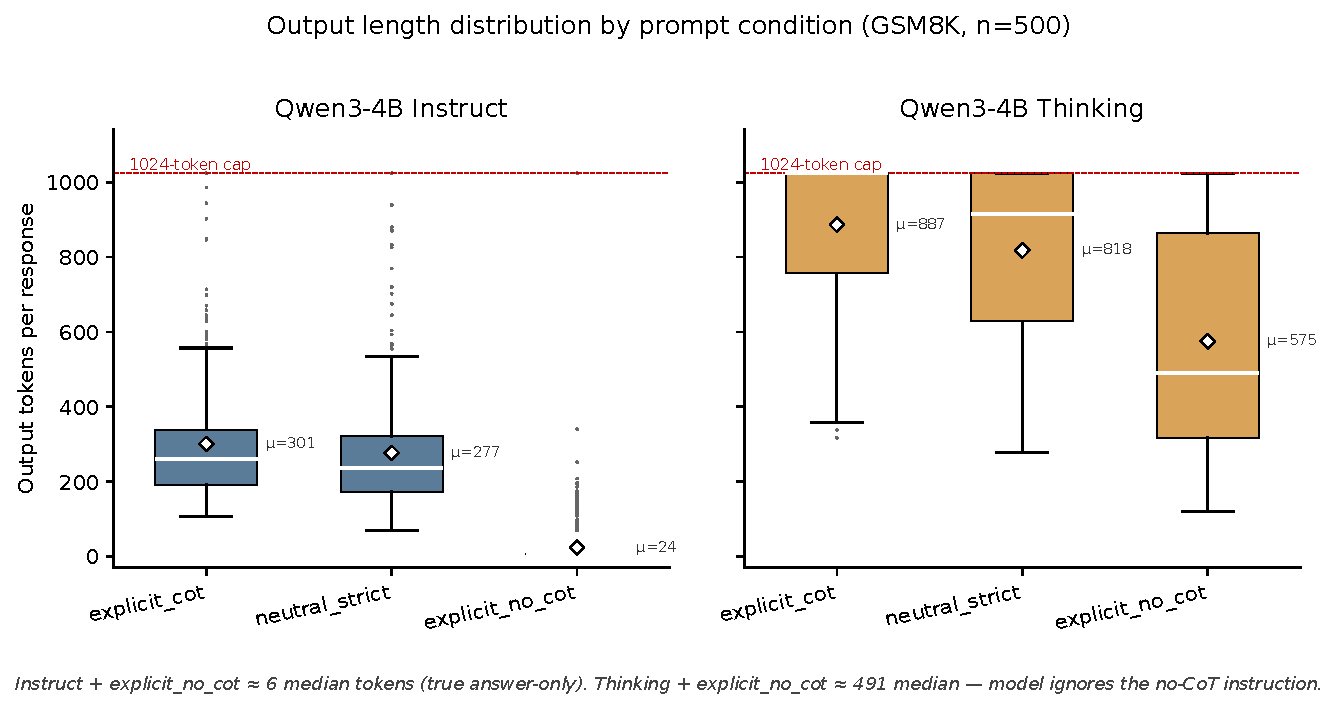
\includegraphics[width=\columnwidth]{figures/fig5_output_lengths.pdf}
  \caption{\textbf{Output-length distributions by prompt condition on GSM8K $n{=}500$.}
  The dashed line marks the 1024-token cap used in baseline generation.
  Qwen3-4B-Instruct approaches an answer-only regime under
  \texttt{explicit\_no\_cot} (mean $\mu=24$ tokens), whereas
  Qwen3-4B-Thinking still produces long continuations in the same condition
  (mean $\mu=575$; median 490.5). The \texttt{neutral\_strict}
  distribution remains close to explicit CoT for Thinking and closer to CoT
  than to no-CoT for Instruct, consistent with the positive HCDS values in
  the main paper.}
  \label{fig:output-length}
\end{figure}

Figure~\ref{fig:output-length} visualizes why \texttt{explicit\_no\_cot}
is a cleaner control for Instruct than for Thinking. For Instruct, the
answer-only directive sharply compresses the length distribution. For
Thinking, the same directive fails to suppress long-form generation, which is
consistent with our interpretation that reasoning is more deeply integrated
and less prompt-conditional in the reasoning-tuned model.

\section{Negative-Control Calibration}
\label{app:negative-control}

A natural concern with HCDS is that it could detect stylistic
differences between prompts --- longer, higher-entropy completions
under neutral than under no-CoT --- rather than reasoning per se.
To address this directly, we ran HCDS on two task families where
multi-step hidden reasoning is implausible:

\begin{itemize}
\item \textbf{Single-step arithmetic} ($n=50$): randomly generated
  questions like ``What is $8 \times 6$?''. Gold answers are
  programmatic.
\item \textbf{Numeric-answer factual lookup} ($n=50$): hand-curated
  well-known facts with verifiable integer answers (``How many
  states are in the US?'', ``In what year did humans first land on
  the Moon?'').
\end{itemize}

We ran the same baseline pipeline (Appendix~\ref{app:hparams}) under
all three prompts on both Qwen3-4B variants and computed the
\emph{latency-only} HCDS variant --- the same single-feature variant
reported on GSM8K in Section~\ref{sec:robustness}. Latency-only is the
most adversarial setting for the stylistic-differences hypothesis,
because it is measured directly from generation timing with no
content-level processing.

\begin{table*}[t]
\centering
\small
\begin{tabular}{llrrr}
\toprule
Task family & Model & $\overline{\mathrm{HCDS}}$ & 95\% CI & $p$ \\
\midrule
GSM8K (reasoning, $n=50$) & Instruct & $+1.79$ & $[+1.58, +2.03]$ & $2.6 \times 10^{-19}$ \\
GSM8K (reasoning, $n=50$) & Thinking & $+0.40$ & $[+0.21, +0.61]$ & $3.9 \times 10^{-4}$ \\
\midrule
Arithmetic (no reasoning, $n=50$) & Instruct & $+0.80$ & $[+0.53, +1.27]$ & $5.0 \times 10^{-4}$ \\
Arithmetic (no reasoning, $n=50$) & Thinking & $-0.11$ & $[-0.23, +0.01]$ & $0.10$ \\
Factual lookup (no reasoning, $n=50$) & Instruct & $+1.18$ & $[+0.92, +1.50]$ & $7.6 \times 10^{-10}$ \\
Factual lookup (no reasoning, $n=50$) & Thinking & $-0.15$ & $[-0.28, -0.03]$ & $0.03$ \\
\bottomrule
\end{tabular}
\caption{Latency-only HCDS on GSM8K (where reasoning is required)
compared to two negative-control task families (where multi-step
hidden reasoning is implausible). Thinking calibrates to
$\approx 0$ on both negative controls; Instruct shows partial
calibration with roughly 45\%--66\% of the GSM8K HCDS persisting on
tasks that require no reasoning. The interpretation is summarized in
Section~\ref{sec:discussion}.}
\label{tab:negative-control}
\end{table*}

The interpretation appears in Section~\ref{sec:discussion}: the
Thinking-model HCDS calibrates essentially to zero on both negative
controls (despite Thinking still emitting hundreds of tokens of
internal reasoning on ``$8 \times 6$''-type questions), so the GSM8K
Thinking HCDS of $+0.40$ is attributable to reasoning- or
prompt-invariance-driven latency differences rather than to a
``Thinking talks more under neutral than under no-CoT'' confound.
The Instruct HCDS only partially calibrates, indicating that the
latency-only HCDS for Instruct is a hybrid of reasoning-induced
timing and stylistic prompt-compliance. We estimate the
reasoning-attributable component of the Instruct GSM8K HCDS as
roughly $+1.0$ in absolute terms (GSM8K minus the non-reasoning
baseline of $\sim$0.8--1.2). A full multi-feature negative-control
calibration --- adding entropy, paraphrase, perturbation, and
mechanistic features on the same task families --- is the next
robustness check we plan.

\paragraph{Parser note.}
Accuracy is not used as an HCDS feature, but the Thinking model
occasionally fails to produce a $\boxed{}$-delimited answer on
negative-control questions because it truncates at the 1024-token cap
before finishing its self-reflection. The numeric parser then falls
back to ``last number in text,'' which can produce spurious low
accuracy (e.g., Thinking writes $\sim$1000 tokens about ``50 states
since the admission of Hawaii in 1959'' and the parser reports the
answer as 1959). This does not affect HCDS computation
(latency-per-token does not depend on parsed accuracy), and is itself
further evidence of Thinking's prompt-invariant reasoning behavior.

\section{Length-Matched HCDS}
\label{app:length-matched}

\begin{figure}[!t]
\centering
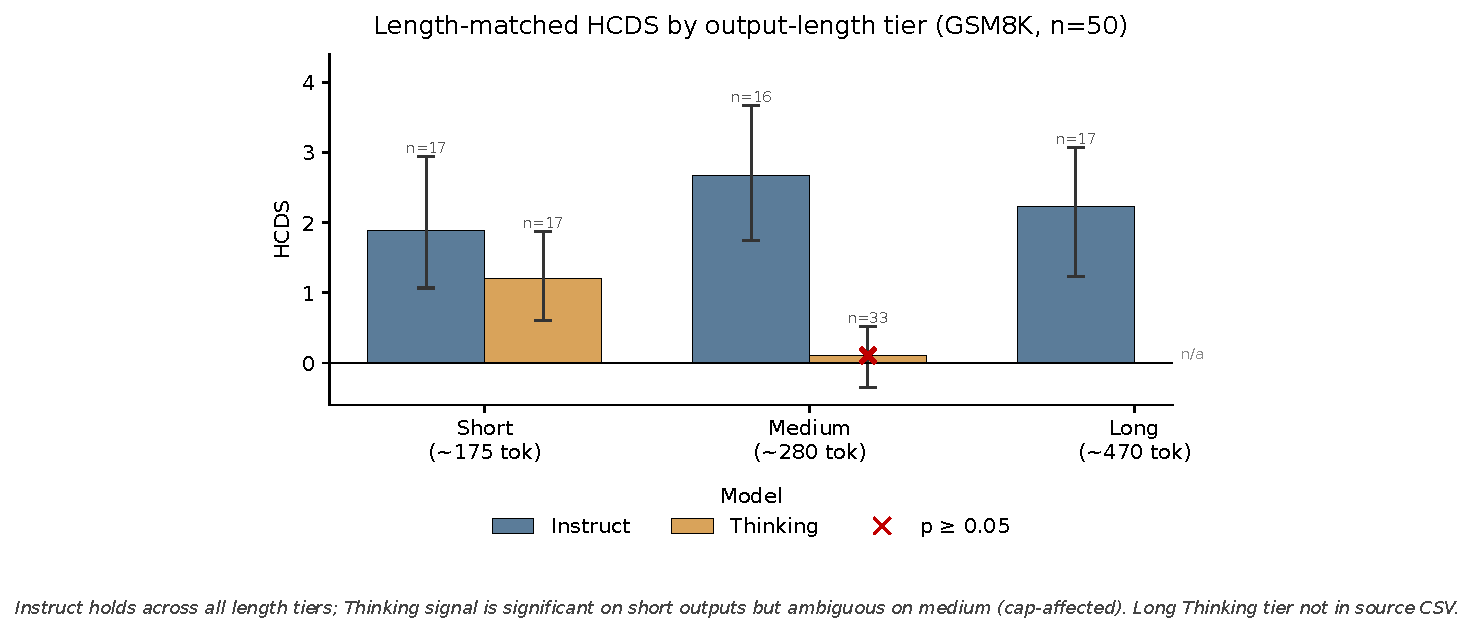
\includegraphics[width=\columnwidth]{figures/fig3_length_matched.pdf}
\caption{\textbf{Length-matched HCDS by output-length tier on GSM8K $n{=}50$.}
Instruct remains positive across short, medium, and long tiers. Thinking is
positive on short outputs but ambiguous on the medium tier ($p=0.65$, marked
with $\times$). No Thinking long-tier bar is shown because the source CSV did
not include it.}
\label{fig:length}
\end{figure}

We split GSM8K $n{=}50$ into output-length tertiles (using the
\textit{explicit\_cot} output length as the binning variable) and
recomputed HCDS within each tier. Figure~\ref{fig:length} and
Table~\ref{tab:length-matched} show
that the Instruct effect is positive and significant in every tier,
while the Thinking effect weakens in the medium tier, consistent
with our reading that medium-length Thinking outputs are most affected
by the 1024-token cap.

\begin{table}[!htbp]
\caption{Length-matched HCDS by output-length tier on GSM8K $n{=}50$.
Tier boundaries are tertiles of explicit-CoT output length per model.
The thinking-long tier is omitted because the source CSV
(\texttt{hcds\_length\_matched.csv}) did not include it; the
\texttt{long} bin for Thinking is dominated by cap-truncated runs and
is left to future work.}
\label{tab:length-matched}
\centering
\small
\setlength{\tabcolsep}{3pt}
\renewcommand{\arraystretch}{1.08}
\begin{tabular}{@{}llrrrr@{}}
\toprule
Model & Tier & $n$ & CoT tok & HCDS & $p$ \\
\midrule
Instruct & short  & 17 & 175.5  & $+1.890$ & $9.4\mathrm{e}{-4}$ \\
Instruct & medium & 16 & 279.8  & $+2.673$ & $1.1\mathrm{e}{-4}$ \\
Instruct & long   & 17 & 472.4  & $+2.224$ & $4.3\mathrm{e}{-4}$ \\
Thinking & short  & 17 & 716.6  & $+1.205$ & $2.1\mathrm{e}{-3}$ \\
Thinking & medium & 33 & 1013.2 & $+0.106$ & $0.65$ \\
\bottomrule
\end{tabular}
\end{table}

\section{Mechanistic Anchor Methodology --- Full Details}
\label{app:mech-details}

This appendix expands the brief methodology summary in
Section~\ref{sec:results-mech} with the full per-cell details
needed to evaluate or replicate the anchor-suppression analysis.

\paragraph{Anchor selection.}
For each (model, prompt, question) cell, every reasoning step is
scored on three attention-/activation-based proxies, all measured
over the step's generated token positions:
\begin{itemize}
\item \texttt{future\_attention\_mean} --- mean attention paid to this
  step's tokens by all \emph{later} reasoning steps in the trace
  (averaged over all attention layers and heads).
\item \texttt{answer\_attention\_mean} --- mean attention paid to this
  step's tokens by tokens inside the final-answer span.
\item \texttt{activation\_delta\_mean} --- L2 norm of the residual-stream
  delta induced at this step's tokens, averaged over layers $\geq 1$.
\end{itemize}
Each of the three is then z-scored across the trace, and the
unweighted sum gives \texttt{combined\_anchor\_score}. Steps are ranked
by descending score, and the top-\textbf{2} steps are selected as
anchors per cell (\texttt{MECH\_TOP\_ANCHOR\_STEPS=2}).

\paragraph{Intervention layers.}
For each anchor or control step, we identify the four
\emph{step-specific} layers with the highest combined
$\mathrm{answer\_attention\_by\_layer} +
\mathrm{future\_attention\_by\_layer}$, where the per-layer attention
is summed over the step's token positions
(\texttt{MECH\_TOP\_ANCHOR\_LAYERS=4}). Interventions are applied at
exactly these four layers.

\paragraph{Intervention modes (what is suppressed).}
Two intervention modes are run independently per anchor / control:
\begin{itemize}
\item \texttt{residual\_zero}: at each target layer, multiply the
  residual-stream output by $0$ at the step's token positions
  (and only those positions). Other token positions and other
  layers are unchanged.
\item \texttt{attention\_zero}: at each target layer, multiply the
  attention-block output by $0$ at the step's token positions.
\end{itemize}
After the suppression hook is installed, generation resumes from the
prefix \emph{up to and including} the perturbed step, with the same
greedy decoding settings and the intervention max-token cap of 384.
The resulting completion is parsed for the final answer and compared
to the unperturbed baseline; \texttt{intervention\_correct} is the
indicator that the post-intervention prediction matches gold.

\paragraph{Control-step selection.}
After anchors are chosen, control steps are sampled \emph{uniformly
at random without replacement} from the set of non-anchor reasoning
steps in the same trace, with one control step per cell
(\texttt{MECH\_NUM\_CONTROL\_STEPS=1}). The same per-step layer rule
is then used to choose the four target layers for the control. A
fixed run-level seed (17) determines the control-step shuffle, so the
control set is reproducible across reruns. Crucially, controls are
\emph{not} matched on trace position, step length, or step function
--- this is one of the limitations called out in
Section~\ref{sec:limitations}.

\paragraph{Examples included / excluded.}
Anchor analysis is only run when the baseline trace contains at
least one reasoning step with a non-empty
\texttt{generated\_token\_positions} field --- i.e., a step that
spans more than a single boxed answer. Per-cell counts on our two
deep-table runs:

\begin{table}[!htbp]
\centering
\small
\setlength{\tabcolsep}{4pt}
\begin{tabular}{@{}lllrr@{}}
\toprule
Dataset & Model & Prompt & Usable & Excluded \\
\midrule
GSM8K       & Instruct & explicit\_cot     & 50 & 0 \\
GSM8K       & Instruct & explicit\_no\_cot &  4 & 46 \\
GSM8K       & Instruct & neutral\_strict   & 50 & 0 \\
GSM8K       & Thinking & explicit\_cot     & 50 & 0 \\
GSM8K       & Thinking & explicit\_no\_cot & 50 & 0 \\
GSM8K       & Thinking & neutral\_strict   & 50 & 0 \\
\midrule
StrategyQA  & Instruct & explicit\_cot     & 50 & 0 \\
StrategyQA  & Instruct & explicit\_no\_cot &  0 & 50 \\
StrategyQA  & Instruct & neutral\_strict   & 50 & 0 \\
StrategyQA  & Thinking & explicit\_cot     & 50 & 0 \\
StrategyQA  & Thinking & explicit\_no\_cot & 50 & 0 \\
StrategyQA  & Thinking & neutral\_strict   & 49 & 1 \\
\bottomrule
\end{tabular}
\caption{Anchor analysis usability per (dataset, model, prompt)
cell, out of 50 questions each. Across both deep-table runs, 503 of
600 (model $\times$ prompt $\times$ question) cells yield a usable
anchor analysis. Almost all exclusions come from the
\texttt{Instruct $\times$ explicit\_no\_cot} cell, where Instruct
compliantly produces an answer-only output ($\sim$6 tokens, e.g.\
\texttt{\textbackslash boxed\{48\}}) with no separable reasoning steps
for the analysis to run on. The single excluded StrategyQA Thinking
$\times$ neutral\_strict question failed parsing on its anchor
probe.}
\label{tab:anchor-coverage}
\end{table}

\paragraph{Why the Instruct $\times$ \texttt{explicit\_no\_cot} cell
is sparse.} The Instruct model complies with the no-CoT directive
and produces median 6-token outputs (mostly \texttt{\textbackslash boxed\{N\}} alone).
Anchor analysis requires separable reasoning steps; with no reasoning
in the output, there is nothing to anchor. We treat this not as a
methodological failure but as itself informative: it means the
\texttt{Instruct $\times$ \texttt{explicit\_no\_cot}} pole is genuinely
``answer-only'' in a way the Thinking $\times$ \texttt{explicit\_no\_cot}
pole is not (Thinking still produces 50/50 usable anchor cells under
the same prompt --- direct evidence of the prompt-invariance finding
discussed in Section~\ref{sec:discussion}).

\paragraph{Anchor-scoring bias toward late-trace steps.}
Independent investigation showed that the attention-based anchor
score systematically prefers late-trace ``summary'' or
``answer-formulation'' steps in long traces, because those steps
are by construction the ones that downstream tokens attend to most.
Suppressing these post-hoc summary steps is less damaging than
suppressing earlier mid-reasoning computation that downstream tokens
have not yet copied. An optional late-trace position penalty
(\texttt{AJAR\_ANCHOR\_LATE\_PENALTY}) is plumbed through the runner;
the runs reported in this paper use the unpenalised score
(\texttt{penalty\_alpha=0}) to match the original proposal exactly,
and we mark a position-aware re-run as future work
(Section~\ref{sec:limitations}).

\section{Sensitivity to Feature-Subset Weighting}
\label{app:sensitivity}

Because HCDS combines six features with equal weighting in z-scored
space, a natural reviewer concern is whether the headline conclusion
depends on that weighting choice. We address this with a discrete
sensitivity analysis: for each (dataset, model) we recompute HCDS
on every $2^k - 1$ non-empty subset of the $k$ features available
in that dataset's task6 table, and record the fraction of subsets
for which HCDS is positive and significantly positive ($p<0.05$
two-sided one-sample $t$-test).

\begin{table}[!htbp]
\centering
\small
\setlength{\tabcolsep}{4pt}
\begin{tabular}{@{}llrrr@{}}
\toprule
Dataset & Model & Subsets & \% positive & \% sig.\ positive \\
\midrule
GSM8K $n=50$       & Instruct & 63 & 96.8\% & 87.3\% \\
GSM8K $n=50$       & Thinking & 63 & 84.1\% & 47.6\% \\
StrategyQA $n=50$  & Instruct & 14 & 92.9\% & 85.7\% \\
StrategyQA $n=50$  & Thinking & 15 & 93.3\% & 60.0\% \\
GSM8K $n=500$      & Instruct & 63 & 98.4\% & 95.2\% \\
GSM8K $n=500$      & Thinking & 63 & 76.2\% & 69.8\% \\
\bottomrule
\end{tabular}
\caption{HCDS sign and significance coverage across all non-empty
feature subsets per (dataset, model). StrategyQA admits fewer
subsets because the paraphrase- and perturbation-feature pipelines
were not run for it; GSM8K $n=500$ uses partial-feature aware
distance computation where the mechanistic feature is available
only on the $n=50$ subsample.}
\label{tab:sensitivity}
\end{table}

\paragraph{Where the negative-sign subsets fall.} On GSM8K $n=50$,
the only two subsets with negative-sign Instruct HCDS are
(\texttt{mechanistic\_intervention}) alone (HCDS $=0$, degenerate)
and (\texttt{perturbation\_delta}, \texttt{mechanistic\_intervention})
(HCDS $=-0.30$, $p=0.22$ n.s.) --- both are subsets that contain
no behavioral or linguistic features. All ten negative-sign Thinking
subsets exclude both entropy features, exactly consistent with the
entropy-load-bearing finding in Section~\ref{sec:robustness}: the
Thinking pathway depends on token-level entropy as its primary
HCDS-positive signal, and removing entropy collapses the score.

\paragraph{Implications.} The headline conclusion --- HCDS positive,
neutral behavior aligns with explicit CoT --- holds for the large
majority of feature-weight configurations we tested. Equal-weighting
is therefore not load-bearing for the result; almost any non-trivial
weighting that includes the load-bearing features yields the same
sign. The discrete subset coverage is the cheapest sensitivity check
that can be run from the existing task6 tables without additional
model generations; we extend it to continuous weightings next.

\paragraph{Continuous weight sampling.} The subset analysis above
varies feature weights in $\{0,1\}$; to test robustness to arbitrary
continuous weightings we draw $10{,}000$ weight vectors uniformly from
the feature simplex (Dirichlet$(1,\dots,1)$) and recompute HCDS under
the weighted metric $D_w(a,b)=\sqrt{\sum_j w_j (a_j-b_j)^2}$. Because
$\mathrm{HCDS}=D_1-D_2$ and both distances scale by $\sqrt{c}$ under
$w\mapsto cw$, the sign and one-sample $t$-statistic are invariant to
the overall scale, so simplex weights are directly comparable to the
equal weighting of the main text, which the procedure reproduces
exactly as its anchor (GSM8K Instruct $+2.25$, Thinking $+0.48$).
Across the three task families, Instruct HCDS remains positive in
$98.2$--$100\%$ of sampled weightings and significantly positive in
$93.1$--$100\%$; Thinking remains positive in $94.2$--$100\%$ but
significantly positive in only $52.2$--$86.9\%$, localizing the
fragility in the reasoning-tuned model. Uniform simplex sampling places
substantial mass near single-feature corners, making this a
deliberately adversarial test, and the near-universal survival of the
Instruct sign shows the headline result does not depend on the
equal-weighting choice. Equal weighting yields a magnitude near the top
of the sampled distribution --- expected, since it aggregates all six
features rather than concentrating on a few --- but the robustness
claim rests on the weight-independent sign, not the magnitude. We
deliberately do not \emph{optimize} the weights: HCDS is unsupervised,
with no per-question hidden-CoT label, so tuning weights to enlarge the
effect would be circular; equal weighting is retained as a principled
default whose robustness we verify rather than fit.

\section{Joint Anchor Suppression}
\label{app:joint-anchor}

The negative anchor-control contrast on Thinking + \texttt{explicit\_cot}
($-0.275$ in Figure~\ref{fig:anchor}) admits two non-mutually-exclusive
interpretations: distributed causal load (Hypothesis~A) or
attention-based anchor scoring biased toward late-trace summary steps
(Hypothesis~B). To partially disambiguate, we ran a joint-suppression
experiment that targets both top-2 anchor steps \emph{simultaneously}
(union of token positions, union of top-4 step-specific layers) and a
matched joint control that suppresses 2 random non-anchor steps
simultaneously, both with the same two intervention modes
(\texttt{residual\_zero} and \texttt{attention\_zero}) used in the main
results. We re-use the existing baseline traces and anchor selections
from the deep-table run; only the joint interventions are newly
generated. All 50 tasks ran to completion with zero failures.

\begin{table}[!htbp]
\centering
\small
\setlength{\tabcolsep}{4pt}
\begin{tabular}{@{}lrr@{}}
\toprule
Metric & Single (existing) & Joint (new) \\
\midrule
Baseline accuracy             & $0.840$ & $0.840$ \\
Anchor mean accuracy          & $0.735$ & $0.700$ \\
Control mean accuracy         & $0.460$ & $0.580$ \\
\midrule
Anchor drop                   & $0.105$ & $0.140$ \\
Control drop                  & $0.380$ & $0.260$ \\
$\mathrm{anchor\_drop} - \mathrm{control\_drop}$ & $-0.275$ & $-0.120$ \\
\bottomrule
\end{tabular}
\caption{Single-step versus joint-step anchor suppression on
Thinking + \texttt{explicit\_cot} GSM8K $n{=}50$. ``Single'' columns
reproduce the result reported in the main paper (Figure~\ref{fig:anchor});
``Joint'' columns suppress two anchors / two controls simultaneously.
Per-mode breakdown: anchor $\times$ residual\_zero acc $=0.720$,
anchor $\times$ attention\_zero acc $=0.680$, control $\times$
residual\_zero acc $=0.640$, control $\times$ attention\_zero acc
$=0.520$.}
\label{tab:joint-anchor}
\end{table}

\paragraph{What the joint result shows.} The anchor-control contrast
narrows from $-0.275$ to $-0.120$ --- a 56\% reduction toward zero,
but still negative. Two effects drive the change:

\begin{enumerate}
\item \textbf{Joint anchor suppression has a slightly larger effect
  than single} (drop $0.105 \to 0.140$). This is modest support for
  Hypothesis~A: suppressing both anchors together does compound
  causal load somewhat, consistent with reasoning being distributed
  across multiple steps in the Thinking model.
\item \textbf{Matched joint control happens to sample less impactful
  steps on average than the original single random control}
  ($0.380 \to 0.260$). This tells us the original $-0.275$ contrast
  was inflated by random-control variance: a single random
  non-anchor step happened to land on impactful positions more often
  than a sample of two would on average.
\end{enumerate}

\paragraph{Bottom line.} Hypothesis~A (distributed causal load)
receives partial support from the joint experiment; Hypothesis~B
(anchor scoring bias) is not falsified, since even joint suppression
of attention-identified anchors does not overtake matched random
controls. The honest reading is that both effects contribute and the
single-step negative bar in Figure~\ref{fig:anchor} should be read as
a mild rather than dramatic anchor weakness. Position-matched control
selection (rather than purely random non-anchor sampling) and a
gradient-based anchor score that does not preferentially select
late-trace summary steps would both be expected to further narrow
the contrast; we mark these as the priority follow-up mechanistic
experiments.

\end{document}